\chapter{Results}

In this chapter the results of the search for $\PZ\PZ\PGg$ and $\PW\PZ\PGg$ triboson production,
as well as the measurement of the cross section of $\Pp\Pp \to 4\Pl \PGg$ are presented.
This analysis uses the data collected by the CMS experiment during the 2016-2018 period at a centre-of-mass energy of 13\TeV.
The analysis strategy is to search for excess events over the estimated background yield from known Standard Model processes.
Different identification strategies for the photon and several kinematic distributions are explored.

First the statistical tools used for the extraction of the parameters of interest and interpretation are described.
Then the expected result before unblinding will be discussed, and the best strategy selected.
Finally, the observed results will be reported.

\section{Statistical analysis}
\label{sec:statistical_analysis}
A statistical analysis is conducted to assess the presence of the signal process in the observed data,
quantify the significance of the excess over background predictions and measure its cross section.
The statistical inference is performed with the \textsc{Combine Tool} software package~\cite{CMS-NOTE-2011-005,CMS-CAT-23-001}.

\providecommand{\poissonpdf}[2]{\ensuremath{ \frac{{#1}^{#2}}{#2!}e^{-#1} }}

\subsection{Likelihood and nuisance parameters}
The likelihood function is defined as the probability density function for a set of parameters of a model
that quantifies the agreement with a certain set of experimental observables (data).
The model adopted for this analysis defines a signal strength modifier $\mu$,
that multiplies the production cross section of the signal process and leaves all the other processes unchanged.
Each independent source of systematic uncertainty described in Section \ref{sec:systematics} is assigned a nuisance parameter $\theta_i$, and the full set is denoted $\vec\theta$.
They are of no direct interest for this analysis, but must be considered in the fitting procedure to extract correct results.
They enter the model through their probability density function $p_i(\tilde{\theta_i}|\theta_i)$,
which is the probability of measuring a certain value of the parameter given that the true value is $\theta_i$.
Furthermore, the expected yields of background, $b$, and signal, $s$, depend on the value of the nuisance parameters.

The global likelihood function is thus defined as:
\begin{equation}
  \label{eq:likelihood_full}
  \Likelihood(data\, |\, \mu, \vec\theta\,) = \prod_c \Likelihood_c(data\, |\, \mu \cdot s(\vec\theta\,) + b(\vec\theta\,)) \cdot \prod_i p_i(\tilde{\theta_i}\, |\, \theta_i)
\end{equation}
where c runs over all the channels, which are the four data-taking periods (2016preVFP, 2016postVFP, 2017, 2018).
The extraction of the signal strength proceeds through the maximization of the complete likelihood function by varying the parameter of interest $\mu$ and the nuisances.
The $\Likelihood_c$ functions are the PDF of the binned distributions in each channel, and are given by the product of Poisson probabilities for every bin $j$ to observe $n_j$ events:
\begin{equation}
  \label{eq:likelihood_bin}
  \Likelihood_c(data\, |\, \mu \cdot s(\vec\theta\,) + b(\vec\theta\,)) =
                       \prod_j \poissonpdf{\left( \mu \cdot s_j(\vec\theta\,) + b_j(\vec\theta\,) \right)}{n_j}
\end{equation}

\subsection{Treatment of nuisance parameters}
Systematics uncertainties can be categorized into two main classes: the ones that affect only the event yield, and those that have an impact also on the shape of the predicted distributions.
Most of the uncertainties of the first class are parametrized with a log-normal distribution:
\begin{equation}
  \label{eq:lnNdef}
  \Probability(\tilde{\theta}\,|\,\theta) = \frac{1}{\sqrt{2 \pi} \text{ln} k} \cdot \frac{1}{\tilde{\theta}} \cdot \text{exp} \left( -\frac{(\text{ln}(\tilde{\theta}/\theta_m))^2}{2 \text{ln}^2 k} \right)
\end{equation}
which is the distribution of a random variable whose logarithm is normally distributed, with mean $\mu$ = $\text{ln}(\theta_m)$ and standard deviation $\sigma$ = $\text{ln}(k)$.
%% where the parameters $theta_s$ and $k$ can be defined in terms of the mean and standard deviation of a normally distributed variable: $\theta_m = e^{\mu}$ and $k = e^{\sigma}$.
The log-normal is used instead of a Gaussian because it enforces the positive-definite normalization for the nuisance modelled, which is usually multiplying an event yield and thus cannot be negative.

The remaining systematics in the first class are those that represent a background coming from a statistically limited control region, such as the fake leptons and photons.
These are dominated by the statistically uncertainty in the control region and are modelled with a Gamma distribution:
\begin{equation}
  \label{eq:gammadef}
  \Probability(\theta\,|\,N\alpha) = \frac{1}{\Gamma(N) \alpha^N} \theta^{N-1} e^{-\theta/\alpha}
\end{equation}
where $N$ is the number of events in the control region, $\theta$ is the average transfer factor and $\Gamma(x)$ is the Gamma function.

The shape uncertainties of the second class are accounted for by interpolating the event fraction for each bin of three histograms:
the one obtained for the central value, and the two obtained by shifting the nuisance parameter up and down by one standard deviation~\cite{CMS-CAT-23-001}.

\subsection{Quantifying an excess}
To quantify the statistical significance of an excess of events over the background-only hypothesis, the following test statistic is used:
\begin{equation}
  \label{eq:test_statistic}
  t_0 = -2\text{ln} \frac {\Likelihood(data\,|\,0,\widehat{\vec{\theta_0}}\,)} {\Likelihood(data\,|\,\hat\mu,\widehat{\vec\theta}_{\hat\mu})}\,,\quad \text{with}\, \hat\mu \ge 0
\end{equation}

The numerator is evaluated under the background-only hypothesis ($\mu$ = 0), and $\widehat{\vec{\theta_0}}$ is the set of values of nuisance parameters that maximizes it under this null hypothesis.
The denominator is evaluated under the alternative signal + background hypothesis,
and the values $\hat{\mu}$ and $\widehat{\vec{\theta}}_{\hat\mu}$
are those that maximize the likelihood in this hypothesis.
This quantity is positive for a signal-like excess ($\mu$ > 0) and becomes 0 in the absence of an excess ($\mu$ = 0).

The significance of an excess is expressed in terms of the local \textit{p-value}, which is the probability to obtain a value of the test statistic $t_0$ greater than or equal to the one observed in experimental data, under the background-only hypothesis:
\begin{equation}
  \label{eq:pvalue}
  p_0 = \Probability(t_0 \ge t_0^{obs}\, |\, \mu = 0)
\end{equation}
That is, $p_0$ is the probability that a local statistical fluctuation of the background yield
is compatible with the observed data in the background only hypothesis,
at least as much as the signal hypothesis.

The p-value is usually expressed as a \textit{significance} $Z$ using the Gaussian one-sided integral:
\begin{equation}
  \label{eq:significance}
  p_0 = \int_Z^\infty \frac{1}{\sqrt{2\pi}}e^{-x^2/2}dx
\end{equation}

The conventional values of $Z$ = 3$\sigma$ and $Z$ = 5$\sigma$, corresponding to p-values of $1.3 \times 10^{-3}$ and $2.8 \times 10^{-7}$, are used to claim evidence for and the discovery of a new phenomenon respectively.


\subsection{Likelihood scans}
\label{sec:likelihood_scans}
The extraction of the signal strength modifier $\mu$ proceeds through the maximization of the likelihood.
%% as described in Section~\ref{sec:statistical_analysis}.
This procedure can be visualized by scanning the likelihood function for several values of the parameter $\mu$
accounting for the systematic uncertainties affecting the measurement.
For each value the best fit value of the nuisance parameters is computed,
and the resulting value of the likelihood is stored.
The corresponding points are then plotted as a function of $\mu$.

Usually the auxiliary quantity $-2\Delta\ln\Likelihood$ (defined as $t_0$ in Equation~\ref{eq:test_statistic})
is used instead of the likelihood itself.
The width of the its profile is linked to the uncertainty on the estimate of $\mu$ from the fit.
More precisely, the set of values $\{ \mu \mid -2\Delta\ln\Likelihood(\mu) < 1 (4) \}$ corresponds to the 68\usep\% (95\usep\%) confidence interval
in the case of a one-dimensional likelihood fit.

This procedure can also be performed by fixing the values of one or more nuisances instead of allowing them to be fitted by the algorithm.
The effect of fixing the value of one or more parameters is a reduction in the overall width of the likelihood shape.
This difference is ascribed to the effect of the \textit{frozen} parameters.

Nuisance parameters are categorized as follows:
\begin{itemize}
\item \textbf{theory:} uncertainties on the QCD scale, proton PDFs and on the value of \alpS;
%% \item \textbf{data-driven:} uncertainties related to the data-driven estimate of fake lepton or fake photon backgrounds;
\item \textbf{luminosity:} the uncertainty on the integrated luminosity corresponding to the data collected by the CMS experiment;
\item \textbf{experimental:} the other experimental uncertainties, such as the lepton or photon efficiency scale factors or the \pileup{} weight,
      including the uncertainty on the data-driven background prediction;
\item \textbf{statistical:} the remaining uncertainty after freezing all of the nuisances.
\end{itemize}

\subsection{Systematic impacts}
\label{sec:systematic_impacts}
The impact of a given source of systematic is defined as the shift $\Delta\mu$ on the signal strength
induced by fixing the corresponding nuisance parameter $\theta_i$ to its $\pm 1 \sigma$ values,
while profiling the other parameters as normal~\cite{CERN-PH-EP-2014-214}.
This is effectively a measure of the correlation between the $i$-th nuisance and the signal strength,
and is useful for determining which nuisances have the largest effect on the uncertainty.


\section{Comparison of strategies}
As mentioned in Sections \ref{sec:evt_photon_selection} and \ref{sec:FSR_cut},
different approaches are used to select the photon
and results are reported both including and excluding the FSR contribution.

Additionally, several event variables are tested for the final fit to the signal strenght.

The first is the invariant mass of the $\PZ\PZ\PGg$ system.
It is expected to be higher for triboson events where the photon comes from the hard scattering than for FSR.
Additionally, it is expected to be sensitive to Beyond Standard Model (BSM) contributions, expecially in the high-energy tail.

The second variable is the transverse momentum of the photon.
As the $\PZ\PZ\PGg$ mass, it is presumed to be sensitive to BSM physics in the high-momentum tail.

The third option considered is the MVA-based ID working point passed by the photon.
Three bins are defined:
\begin{itemize}
\item \makebox[7em][l]{\bf wp80} The photon passes the \texttt{wp80} working point;
\item \makebox[7em][l]{\bf $\mathrm{wp90} \land \mathrm{!wp80}$} The photon passes \texttt{wp90}, but fails \texttt{wp80};
\item \makebox[7em][l]{\bf None} The photon fails \texttt{wp90};
\end{itemize}
The yield of the simulation is scaled in each bin according to the appropriate scale factors (see Section \ref{sec:photonID}).

This section reports the results for all of the combination of the aforementioned choices of the analysis strategy.

\section{Four lepton channel}
\subsection{Inclusive cross section}
\label{sec:impacts_inclusive}
\providecommand{\impactswidthscale}{0.6}
The \nonprompt photon contribution is estimated using the data-driven approach.
The variable considered is $m_{\PZ\PZ\PGg}$.
The impacts of the systematic uncertainties on the expected results is shown in Figure \ref{fig:inclusive_cutID_phoCR_mZZGloose}.

\begin{figure}
  \centering
  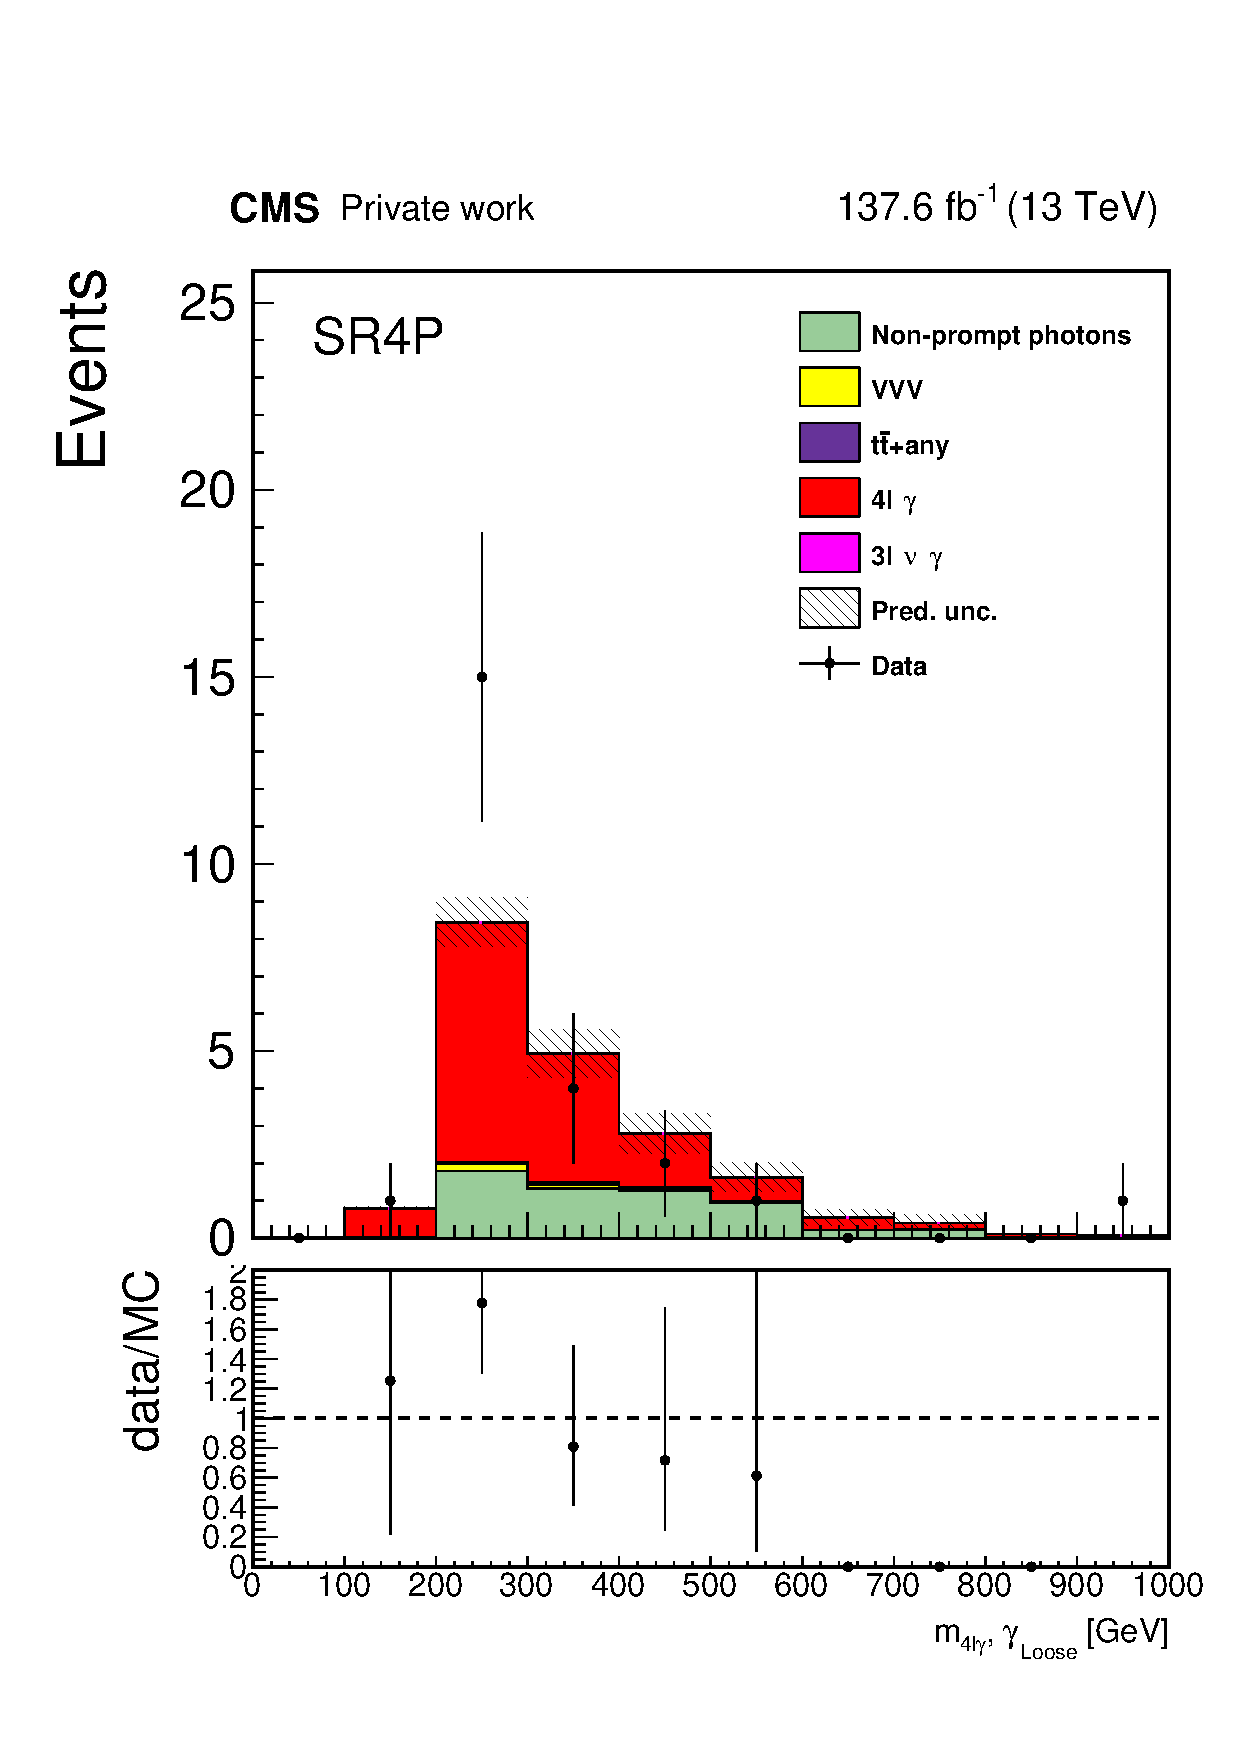
\includegraphics[height=0.33\textheight]{Figures/dataMC/Run2/phoCR/SR4P/SYS_mZZGloose_central_pow.pdf}
  \hfill
  \includegraphics[height=0.33\textheight]{Run2_SR4P_phoCR_lepCR_mZZGloose_impacts.pdf}
  \caption{Distribution and impacts of the systematic uncertainties on the signal strength fit
    on the mass of the $\PZ\PZ\PGg$ system,
    using the Loose working point of the photon cut-based ID.
    The data-driven estimate for \nonprompt photons is used.
    The FSR cut is not applied.
  }
  \label{fig:inclusive_cutID_phoCR_mZZGloose}
\end{figure}

\begin{figure}
  \centering
  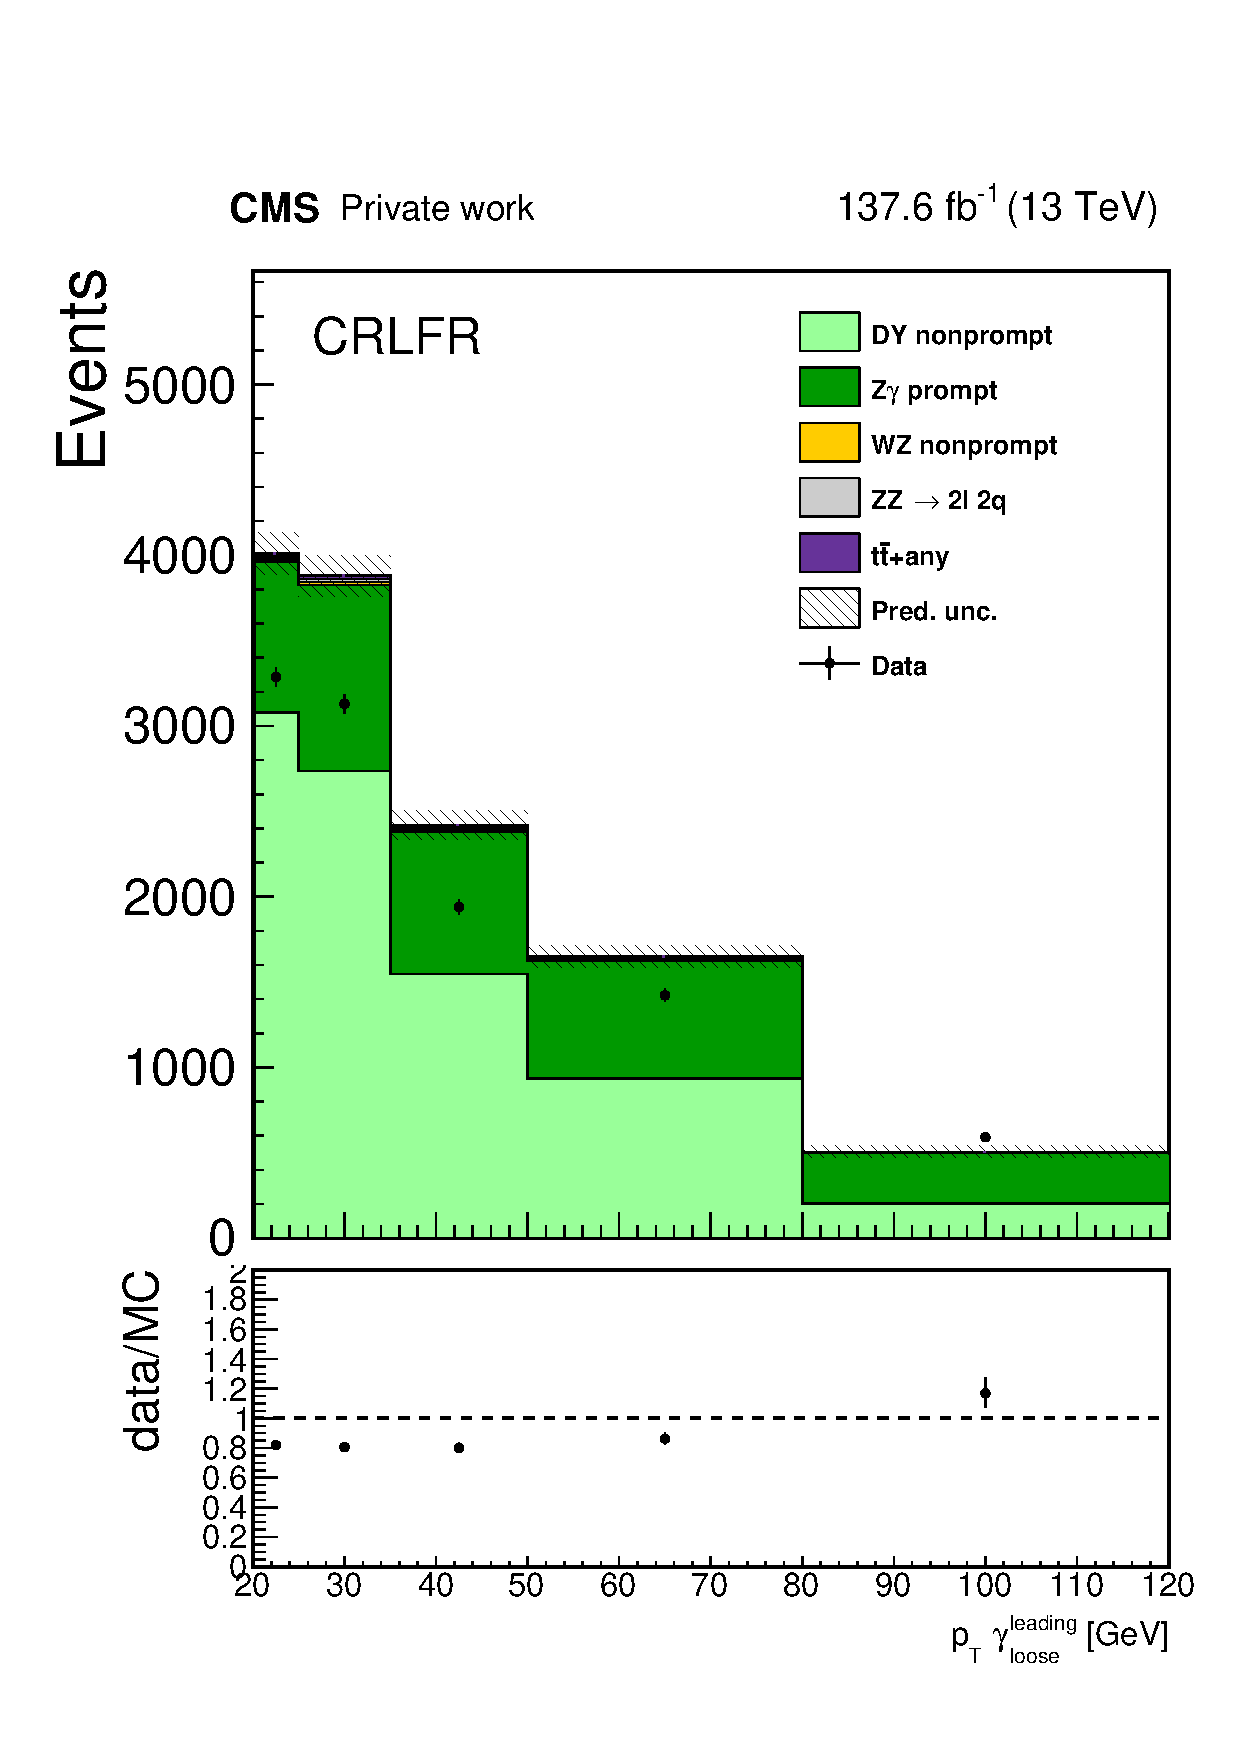
\includegraphics[height=0.33\textheight]{Figures/dataMC/Run2/lepCR/SR4P/lead_loose_pt_pow.pdf}
  \hfill
  \includegraphics[height=0.33\textheight]{Run2_SR4P_phoMC_lepCR_loosept_impacts.pdf}
  \caption{Distribution and impacts of the systematic uncertainties on the signal strength fit
    on the transverse momentum of the photon,
    using the Loose working point of the photon cut-based ID.
    \Nonprompt photons are estimated from simulation.
    The FSR cut is not applied.
  }
  \label{fig:inclusive_cutID_phoMC_loosept}
\end{figure}

\begin{figure}
  \centering
  \includegraphics[height=0.33\textheight]{Figures/dataMC/Run2/lepCR/SR4P/SYS_wp90pt_central_pow.pdf}
  \hfill
  \includegraphics[height=0.33\textheight]{Run2_SR4P_phoMC_lepCR_mZZGwp90_impacts.pdf}
  \caption{Distribution and impacts of the systematic uncertainties on the signal strength fit
    on the mass of the $\PZ\PZ\PGg$ system,
    using the \texttt{wp90} working point of the photon MVA ID.
    \Nonprompt photons are estimated from simulation.
    The FSR cut is not applied.
  }
  \label{fig:inclusive_mvaID_phoMC_mZZGwp90}
\end{figure}

\begin{figure}
  \centering
  \includegraphics[height=0.33\textheight]{Figures/dataMC/Run2/lepCR/SR4P/SYS_wp80pt_central_pow.pdf}
  \hfill
  \includegraphics[height=0.33\textheight]{Run2_SR4P_phoMC_lepCR_mZZGwp80_impacts.pdf}
  \caption{Distribution and impacts of the systematic uncertainties on the signal strength fit
    on the mass of the $\PZ\PZ\PGg$ system,
    using the \texttt{wp80} working point of the photon MVA ID.
    \Nonprompt photons are estimated from simulation.
    The FSR cut is not applied.
  }
  \label{fig:inclusive_mvaID_phoMC_mZZGwp80}
\end{figure}

\begin{figure}
  \centering
  \includegraphics[height=0.33\textheight]{Figures/dataMC/Run2/lepCR/SR4P/SYS_MVAcut_central_pow.pdf}
  \hfill
  \includegraphics[height=0.33\textheight]{Run2_SR4P_phoMC_lepCR_MVAcut_impacts.pdf}
  \caption{Distribution and impacts of the systematic uncertainties on the signal strength fit
    on the yield in the various bins of the photon MVA ID.
    \Nonprompt photons are estimated from simulation.
    The FSR cut is not applied.
  }
  \label{fig:inclusive_kin_phoMC_MVAcut}
\end{figure}


\subsection{Triboson with FSR cut}
\todo{significance with FSR cut}

The significances obtained with the various strategies for the identification of the photon and the estimation of the fake photon background are illustrated in Table~\ref{tab:summary_significances_inclusive}.
\begin{table}
  \centering
  \caption{Summary of the expected signal significance in the inclusive cross section region for different strategies for
    the estimation of the fake photon background,
    photon identification criterion
    and choice of observable for the fit.}
  \label{tab:summary_significances_inclusive}
  \begin{tabular}{llll}
    \toprule
    Photon ID                          & \nonprompt \PGg & Variable         & Significance\\
    \midrule
    \multirow{3}{*}{Cut-based (Loose)} & data-driven     & $m_{\PZ\PZ\PGg}$ & 3.06 $\sigma$\\
                                       & simulation      & $m_{\PZ\PZ\PGg}$ & 3.06 $\sigma$\\
                                       & simulation      & $\pt^\PGg$       & 3.20 $\sigma$\\
    \multirow{2}{*}{MVA ({\tt wp90})}  & simulation      & $m_{\PZ\PZ\PGg}$ & 3.34 $\sigma$\\
                                       & simulation      & $\pt^\PGg$       & 3.35 $\sigma$\\
    MVA ({\tt wp90})                   & simulation      & $m_{\PZ\PZ\PGg}$ & 3.26 $\sigma$\\
    \hline
    Kinematic                          & simulation      & MVA score        & 3.32 $\sigma$\\
    \bottomrule
  \end{tabular}
\end{table}

\begin{table}
  \centering
  \caption{Summary of the expected signal significance in the triboson fiducial region for the different strategies for
    the estimation of the fake photon background,
    photon identification criterion
    and choice of observable for the fit.}
  \label{tab:summary_significances_FSRcut}
  \begin{tabular}{llll}
    \toprule
    Photon ID                          & \nonprompt \PGg & Variable         & Significance\\
    \midrule
    \multirow{3}{*}{Cut-based (Loose)} & data-driven     & $m_{\PZ\PZ\PGg}$ & X $\sigma$\\
                                       & simulation      & $m_{\PZ\PZ\PGg}$ & X $\sigma$\\
                                       & simulation      & $\pt^\PGg$       & X $\sigma$\\
    \hline
    \multirow{2}{*}{MVA ({\tt wp90})}  & simulation      & $m_{\PZ\PZ\PGg}$ & X $\sigma$\\
                                       & simulation      & $\pt^\PGg$       & X $\sigma$\\
    \hline
    MVA ({\tt wp90})                   & simulation      & $m_{\PZ\PZ\PGg}$ & X $\sigma$\\
    \hline
    Kinematic                          & simulation      & MVA score        & X $\sigma$\\
    \bottomrule
  \end{tabular}
\end{table}


\subsection{Likelihood scans inclusive}
\todo{temp name}
% Likelihood scans with nuisance groups without the FSR cut
\label{sec:likelihood_scans_inclusive}
The extraction of the signal strength modifier $\mu$ proceeds through the maximisation of the likelihood,
as described in Section~\ref{sec:statistical_analysis}.
This procedure can be visualised by scanning the likelihood function for several values of the parameter $\mu$ while profiling the nuisance parameters.
For each value the best fit value of the nuisance parameters is computed,
and the resulting value of the likelihood is stored.
These points are then plotted as a function of $\mu$.

Usually the auxiliary quantity $-2\Delta\text{ln}\Likelihood$ (defined as $t_0$ in Equation~\ref{eq:test_statistic})
is used instead of the likelihood itself.
The width of the its profile is linked to the uncertainty on the estimate of $\mu$ from the fit.
More precisely, the set of values $\{ \mu / -2\Delta\text{ln}\Likelihood(\mu) < 1 (4) \}$ corresponds to the 68\usep\% (95\usep\%) confidence interval.

This procedure can also be performed by fixing the values of one or more nuisances instead of allowing them to be fitted by the algorithm.
The effect of fixing the value of one or more parameters is a reduction in the width of the likelihood shape.
This difference is ascribed to the effect of the frozen parameters.

Four groups of parameters are used in the following results:
\begin{itemize}
\item \textbf{theory:} uncertainties on the QCD scale, proton PDFs and on the value of \alpS;
\item \textbf{data-driven:} uncertainties related to the data-driven estimate of fake lepton or fake photon backgrounds;
\item \textbf{luminosity:} the uncertainty on the integrated luminosity corresponding to the data collected by the CMS experiment;
\item \textbf{others:} remaining experimental uncertainties, such as the lepton or photon efficiency scale factors or the \pileup weight;
\end{itemize}

\begin{figure}
  \centering
  \includegraphics[height=.33\textheight]{Figures/dataMC/Run2/phoCR/SR4P/SYS_mZZGloose_central_pow_\dataMCblind .pdf}
  \hfill
  \includegraphics[height=.33\textheight]{Figures/combine/inclusive/scan_\expobs_Run2_SR4P_phoCR_lepCR_mZZGloose.pdf}
  \caption{\captionScan{mass of the $\PZ\PZ\PGg$ system}{Loose}{cut-based ID}{d}{not }}
  \label{fig:scan_Run2_SR4P_phoCR_lepCR_mZZGloose}
\end{figure}

\begin{figure}
  \centering
  \includegraphics[height=.33\textheight]{Figures/dataMC/Run2/lepCR/SR4P/SYS_loosept_central_pow_\dataMCblind .pdf}
  \hfill
  \includegraphics[height=.33\textheight]{Figures/combine/inclusive/scan_\expobs_Run2_SR4P_phoMC_lepCR_mZZGloose.pdf}
  \caption{\captionScan{mass of the $\PZ\PZ\PGg$ system}{Loose}{cut-based ID}{s}{not }}
  \label{fig:scan_Run2_SR4P_phoMC_lepCR_mZZGloose}
\end{figure}

\begin{figure}
  \centering
  \includegraphics[height=0.33\textheight]{Figures/dataMC/Run2/lepCR/SR4P/SYS_mZZGwp90_central_pow_\dataMCblind .pdf}
  \hfill
  \includegraphics[height=.33\textheight]{Figures/combine/inclusive/scan_\expobs_Run2_SR4P_phoMC_lepCR_mZZGwp90.pdf}
  \caption{\captionScan{mass of the $\PZ\PZ\PGg$ system}{\texttt{wp90}}{MVA ID}{s}{not }}
  \label{fig:scan_Run2_SR4P_phoMC_lepCR_mZZGwp90}
\end{figure}

\begin{figure}
  \includegraphics[height=0.33\textheight]{Figures/dataMC/Run2/lepCR/SR4P/SYS_mZZGwp80_central_pow_\dataMCblind .pdf}
  \hfill
  \centering
  \includegraphics[height=.33\textheight]{Figures/combine/inclusive/scan_\expobs_Run2_SR4P_phoMC_lepCR_mZZGwp80.pdf}
  \caption{\captionScan{mass of the $\PZ\PZ\PGg$ system}{\texttt{wp80}}{MVA ID}{s}{not }}
  \label{fig:scan_Run2_SR4P_phoMC_lepCR_mZZGwp80}
\end{figure}

\begin{figure}
  \centering
  \includegraphics[height=.33\textheight]{Figures/dataMC/Run2/lepCR/SR4P/SYS_wp90pt_central_pow_\dataMCblind .pdf}
  \hfill
  \includegraphics[height=.33\textheight]{Figures/combine/inclusive/scan_\expobs_Run2_SR4P_phoMC_lepCR_wp90pt.pdf}
  \caption{\captionScan{transverse momentum of the photon}{\texttt{wp90}}{MVA ID}{s}{not }}
  \label{fig:scan_Run2_SR4P_phoMC_lepCR_wp90pt}
\end{figure}

\begin{figure}
  \centering
  \includegraphics[height=.33\textheight]{Figures/dataMC/Run2/lepCR/SR4P/SYS_MVAcut_central_pow_\dataMCblind .pdf}
  \hfill
  \includegraphics[height=.33\textheight]{Figures/combine/inclusive/scan_\expobs_Run2_SR4P_phoMC_lepCR_MVAcut.pdf}
  \caption{Likelihood scan for the signal strength parameter
    on the yield in the various bins of the photon MVA ID.
    \descriptionFakePhoton{s}.
    The FSR cut is not applied.
    The effect of groups of nuisance parameters on the uncertainty is assessed by sequentially fixing their value in the fit.
  }
  \label{fig:scan_Run2_SR4P_phoMC_lepCR_MVAcut}
\end{figure}

The uncertainty on the signal strength due to the statistics is between 0.35 and 0.50,
and is by far the largest contribution to the total.
This feature is observed for all of the strategies tested here.
The other groups of systematics have much lower impacts.
The theoretical uncertainties are around 0.03-0.05,
while the effect of the luminosity is around 0.03
and the rest of the experimental uncertainties amount to 0.06-0.08 of the signal strength.
The data-driven estimate, when split of the other experimental uncertainties,
adds an undertainty of 0.05-0.08 on the signal strength when estimating the fake photon background
with the data-driven method (Figure~\ref{fig:scan_Run2_SR4P_phoCR_lepCR_mZZGloose}).

\note{Temp}
The signal sample has a cross section of 22.02\usep{}fb, as reported in Table~\ref{tab:listofsamples}.
Assuming a signal strength of
$1.000^{+0.480}_{-0.406}$,
as extracted from
\todo{best strategy}, % TEMP MVAcut
the measured cross section for the production of $\Pp\Pp \to 4\Pl\PGg$ ($\Pl = \Pe,\,\PGm$) at a centre-of-mass energy of $13\TeV$ is
$22.02^{+10.57}_{-8.94}\usep\text{fb}$.


\section{Yields and kinematic distributions}
\label{sec:yields}
After the selections described in Section \ref{sec:event_selection}, the event yields are extracted for signal and backgrounds for each of the four periods of \Run2, for the signal and control regions.

\subsection{Four lepton channel}
The pre-fit yields for the signal and background processes for the signal region
with four leptons passing the tight selection and a photon passing the cut-based ID (SR4P\_1P),
can be seen in Table \ref{tab:Run2_SR4P_phoCR_lepCR} (Table~\ref{tab:Run2_SR4P_phoMC_lepCR})
when using the data-driven (simulation) to estimate tha fake photon background.
Alternatively, the expected yields obtained using the
working point \texttt{wp90} of the MVA ID are shown in Table~\ref{tab:Run2_SR4P_phoMC_lepCR_wp90}.

Additional tables, including also the observed number of data events, are provided
for the fake photon application region (Table \ref{tab:yields_Run2_CR4P_1F_lepCR}),
and for the fake lepton application regions (Tables \ref{tab:yields_Run2_CR3P1F_1P} and \ref{tab:yields_Run2_CR2P2F_1P}).

The yields in the triboson fiducial region are shown
in Table~\ref{tab:yield_SR4P_1P_FSRcut_Loose} for the Loose working point of the cut-based ID,
and in Table~\ref{tab:yield_SR4P_1P_FSRcut_wp90} when using the \texttt{wp80} of the MVA ID instead.

\begin{table}
  \caption{Yields from the signal region SR4P\_1P, with four leptons passing the tight selection and a photon passing the cut-based ID.
  The \nonprompt and misidentified photons are estimated with the data-driven method
  and thus only the events containing a prompt generated photon are included from the main background samples.
  }
  \label{tab:Run2_SR4P_phoCR_lepCR}
  % Note: this is from the variable mZZGloose
  \resizebox{\textwidth}{!}{%
  \begin{tabular}{lccccc}
    \toprule
    {}                            & 2016preVFP         & 2016postVFP        & 2017               & 2018               & \Run2               \\
    \midrule
    $\PZ\PZ\PGg\to4\Pl\PGg$       &  1.962 $\pm$ 0.047 &  1.714 $\pm$ 0.040 &  4.021 $\pm$ 0.100 &  5.864 $\pm$ 0.142 &  13.561 $\pm$ 0.184 \\
    $\Pg\Pg\to\PZ\PZ\to4\Pe$      &  0.031 $\pm$ 0.001 &  0.030 $\pm$ 0.001 &  0.076 $\pm$ 0.002 &  0.104 $\pm$ 0.003 &   0.240 $\pm$ 0.004 \\
    $\Pg\Pg\to\PZ\PZ\to2\Pe2\PGm$ &  0.063 $\pm$ 0.003 &  0.057 $\pm$ 0.002 &  0.069 $\pm$ 0.003 &  0.104 $\pm$ 0.004 &   0.292 $\pm$ 0.006 \\
    $\Pg\Pg\to\PZ\PZ\to4\PGm$     &  0.056 $\pm$ 0.001 &  0.046 $\pm$ 0.001 &  0.117 $\pm$ 0.003 &  0.159 $\pm$ 0.004 &   0.378 $\pm$ 0.005 \\
    $\PZ\PZ\PZ$                   &  0.007 $\pm$ 0.005 &  0.000 $\pm$ 0.000 &  0.017 $\pm$ 0.008 &  0.029 $\pm$ 0.010 &   0.053 $\pm$ 0.014 \\
    $\PQt\PAQt\PZ$+jets           &  0.011 $\pm$ 0.002 &  0.010 $\pm$ 0.002 &  0.036 $\pm$ 0.005 &  0.041 $\pm$ 0.006 &   0.098 $\pm$ 0.009 \\
    Fake photons                  &  1.357 $\pm$ 0.655 &  1.011 $\pm$ 0.509 &  1.368 $\pm$ 0.519 &  2.451 $\pm$ 0.691 &   6.187 $\pm$ 1.198 \\
    $\PW\PZ\PZ$                   &  0.000 $\pm$ 0.000 &  0.021 $\pm$ 0.012 &  0.016 $\pm$ 0.015 &  0.065 $\pm$ 0.027 &   0.102 $\pm$ 0.033 \\
    $\PW\PW\PZ$                   &  0.000 $\pm$ 0.000 &  0.040 $\pm$ 0.040 &  0.041 $\pm$ 0.041 &  0.082 $\pm$ 0.058 &   0.163 $\pm$ 0.082 \\
    \noalign{\vspace{.3ex}}\hline\noalign{\vspace{.3ex}}
    Total                         &  3.488 $\pm$ 0.656 &  2.927 $\pm$ 0.512 &  5.759 $\pm$ 0.531 &  8.900 $\pm$ 0.709 &  21.074 $\pm$ 1.215 \\
    \bottomrule
  \end{tabular}
  }
\end{table}

\begin{table}
  \caption{Yields from the signal region SR4P\_1P, with four leptons passing the tight selection and a photon passing the cut-based ID.
    The \nonprompt and misidentified photons are taken from the simulation.
  }
  \label{tab:Run2_SR4P_phoMC_lepCR}
  % Note: this is from the variable mZZGloose
  \resizebox{\textwidth}{!}{%
  \begin{tabular}{lccccc}
    \toprule
    {}                            & 2016preVFP          & 2016postVFP       & 2017               & 2018               & \Run2               \\
    \midrule
    $\PZ\PZ\PGg\to4\Pl\PGg$       &  1.962 $\pm$ 0.047 &  1.714 $\pm$ 0.040 &  4.021 $\pm$ 0.100 &  5.864 $\pm$ 0.142 &  13.561 $\pm$ 0.184 \\
    $\PQq\PAQq\to\PZ\PZ\to4\Pl$   &  0.243 $\pm$ 0.011 &  0.210 $\pm$ 0.009 &  0.610 $\pm$ 0.018 &  0.858 $\pm$ 0.025 &   1.921 $\pm$ 0.034 \\
    $\Pg\Pg\to\PZ\PZ\to4\Pe$      &  0.036 $\pm$ 0.001 &  0.035 $\pm$ 0.001 &  0.088 $\pm$ 0.002 &  0.124 $\pm$ 0.003 &   0.283 $\pm$ 0.004 \\
    $\Pg\Pg\to\PZ\PZ\to2\Pe2\PGm$ &  0.077 $\pm$ 0.003 &  0.070 $\pm$ 0.003 &  0.086 $\pm$ 0.003 &  0.127 $\pm$ 0.005 &   0.360 $\pm$ 0.007 \\
    $\Pg\Pg\to\PZ\PZ\to4\PGm$     &  0.065 $\pm$ 0.001 &  0.054 $\pm$ 0.001 &  0.139 $\pm$ 0.003 &  0.192 $\pm$ 0.005 &   0.449 $\pm$ 0.006 \\
    $\PZ\PZ\PZ$                   &  0.007 $\pm$ 0.005 &  0.003 $\pm$ 0.003 &  0.021 $\pm$ 0.009 &  0.050 $\pm$ 0.014 &   0.082 $\pm$ 0.017 \\
    $\PW\PZ\PZ$                   &  0.008 $\pm$ 0.008 &  0.028 $\pm$ 0.014 &  0.038 $\pm$ 0.020 &  0.088 $\pm$ 0.031 &   0.163 $\pm$ 0.041 \\
    $\PQt\PAQt\PZ$+jets           &  0.012 $\pm$ 0.003 &  0.011 $\pm$ 0.002 &  0.048 $\pm$ 0.006 &  0.054 $\pm$ 0.007 &   0.124 $\pm$ 0.010 \\
    Fake leptons                  &  0.047 $\pm$ 0.066 &  0.000 $\pm$ 0.000 &  0.089 $\pm$ 0.119 &  0.117 $\pm$ 0.091 &   0.253 $\pm$ 0.164 \\
    $\PW\PW\PZ$                   &  0.000 $\pm$ 0.000 &  0.040 $\pm$ 0.040 &  0.041 $\pm$ 0.041 &  0.082 $\pm$ 0.058 &   0.163 $\pm$ 0.082 \\
    Total                         &  2.458 $\pm$ 0.082 &  2.164 $\pm$ 0.059 &  5.181 $\pm$ 0.164 &  7.557 $\pm$ 0.183 &  17.360 $\pm$ 0.266 \\
    \noalign{\vspace{.3ex}}\hline\noalign{\vspace{.3ex}}
    Total                         &  3.488 $\pm$ 0.656 &  2.927 $\pm$ 0.512 &  5.759 $\pm$ 0.531 &  8.900 $\pm$ 0.709 &  21.074 $\pm$ 1.215 \\
    \bottomrule
  \end{tabular}
  }
\end{table}

\begin{table}
  \caption{Yields from the signal region SR4P\_1P, with four leptons passing the tight selection
  and a photon passing the \texttt{wp90} of the MVA based ID.
  The \nonprompt and misidentified photons are taken from the simulation.
  }
  \label{tab:Run2_SR4P_phoMC_lepCR_wp90}
  % Note: this is from the variable mZZGloose
  \resizebox{\textwidth}{!}{%
  \begin{tabular}{lccccc}
    \toprule
    {}                            & 2016preVFP          & 2016postVFP       & 2017               & 2018               & \Run2               \\
    \midrule
    $\PZ\PZ\PGg\to4\Pl\PGg$       &  2.026 $\pm$ 0.047 &  1.781 $\pm$ 0.041 &  4.294 $\pm$ 0.103 &  6.126 $\pm$ 0.143 & 14.227 $\pm$ 0.187 \\
    $\PQq\PAQq\to\PZ\PZ\to4\Pl$   &  0.192 $\pm$ 0.009 &  0.158 $\pm$ 0.008 &  0.452 $\pm$ 0.015 &  0.652 $\pm$ 0.022 &  1.453 $\pm$ 0.029 \\
    $\Pg\Pg\to\PZ\PZ\to4\Pe$      &  0.036 $\pm$ 0.001 &  0.034 $\pm$ 0.001 &  0.090 $\pm$ 0.002 &  0.120 $\pm$ 0.003 &  0.280 $\pm$ 0.004 \\
    $\Pg\Pg\to\PZ\PZ\to2\Pe2\PGm$ &  0.076 $\pm$ 0.003 &  0.068 $\pm$ 0.003 &  0.086 $\pm$ 0.003 &  0.131 $\pm$ 0.005 &  0.361 $\pm$ 0.007 \\
    $\Pg\Pg\to\PZ\PZ\to4\PGm$     &  0.066 $\pm$ 0.001 &  0.053 $\pm$ 0.001 &  0.141 $\pm$ 0.003 &  0.189 $\pm$ 0.004 &  0.449 $\pm$ 0.006 \\
    $\PZ\PZ\PZ$                   &  0.010 $\pm$ 0.006 &  0.003 $\pm$ 0.003 &  0.023 $\pm$ 0.009 &  0.040 $\pm$ 0.012 &  0.076 $\pm$ 0.016 \\
    $\PQt\PAQt\PZ$+jets           &  0.014 $\pm$ 0.003 &  0.012 $\pm$ 0.002 &  0.045 $\pm$ 0.006 &  0.057 $\pm$ 0.007 &  0.129 $\pm$ 0.010 \\
    Fake leptons                  &  0.045 $\pm$ 0.066 &  0.103 $\pm$ 0.117 &  0.107 $\pm$ 0.118 &  0.022 $\pm$ 0.081 &  0.276 $\pm$ 0.196 \\
    $\PW\PZ\PZ$                   &  0.000 $\pm$ 0.000 &  0.020 $\pm$ 0.012 &  0.063 $\pm$ 0.022 &  0.076 $\pm$ 0.029 &  0.159 $\pm$ 0.038 \\
    $\PW\PW\PZ$                   &  0.000 $\pm$ 0.000 &  0.000 $\pm$ 0.000 &  0.040 $\pm$ 0.040 &  0.080 $\pm$ 0.057 &  0.121 $\pm$ 0.070 \\
    \noalign{\vspace{.3ex}}\hline\noalign{\vspace{.3ex}}
    Total                         &  2.464 $\pm$ 0.082 &  2.233 $\pm$ 0.124 &  5.342 $\pm$ 0.165 &  7.493 $\pm$ 0.178 & 17.532 $\pm$ 0.285 \\
    \bottomrule
  \end{tabular}
  }
\end{table}

\begin{table}
\caption{Yields from the fake photon application region CR4P\_1F, with four leptons passing the tight selection and a photon passing the VeryLoose ID but failing the cut-based ID Loose.}
\label{tab:yields_Run2_CR4P_1F_lepCR}
\resizebox{\textwidth}{!}{%
  \begin{tabular}{lccccc}
    \toprule
    {}                            & 2016preVFP         & 2016postVFP        & 2017               & 2018                & \Run2               \\
    \midrule
    $\PZ\PZ\PGg\to4\Pl\PGg$       &  0.302 $\pm$ 0.019 &  0.294 $\pm$ 0.017 &  0.837 $\pm$ 0.047 &   1.191 $\pm$ 0.064 &   2.623 $\pm$ 0.083 \\
    $\PQq\PAQq\to\PZ\PZ\to4\Pl$   &  2.400 $\pm$ 0.033 &  2.283 $\pm$ 0.030 &  6.428 $\pm$ 0.058 &   9.507 $\pm$ 0.084 &  20.617 $\pm$ 0.111 \\
    $\Pg\Pg\to\PZ\PZ\to4\Pe$      &  0.060 $\pm$ 0.001 &  0.059 $\pm$ 0.001 &  0.168 $\pm$ 0.003 &   0.258 $\pm$ 0.005 &   0.546 $\pm$ 0.006 \\
    $\Pg\Pg\to\PZ\PZ\to2\Pe2\PGm$ &  0.157 $\pm$ 0.004 &  0.158 $\pm$ 0.004 &  0.224 $\pm$ 0.005 &   0.322 $\pm$ 0.008 &   0.860 $\pm$ 0.011 \\
    $\Pg\Pg\to\PZ\PZ\to4\PGm$     &  0.107 $\pm$ 0.002 &  0.092 $\pm$ 0.002 &  0.253 $\pm$ 0.004 &   0.385 $\pm$ 0.006 &   0.837 $\pm$ 0.008 \\
    $\PZ\PZ\PZ$                   &  0.039 $\pm$ 0.011 &  0.025 $\pm$ 0.011 &  0.067 $\pm$ 0.016 &   0.069 $\pm$ 0.019 &   0.200 $\pm$ 0.030 \\
    $\PW\PZ\PZ$                   &  0.064 $\pm$ 0.022 &  0.071 $\pm$ 0.023 &  0.120 $\pm$ 0.034 &   0.120 $\pm$ 0.038 &   0.376 $\pm$ 0.060 \\
    $\PW\PW\PZ$                   &  0.048 $\pm$ 0.048 &  0.046 $\pm$ 0.046 &  0.000 $\pm$ 0.000 &   0.036 $\pm$ 0.036 &   0.131 $\pm$ 0.076 \\
    $\PQt\PAQt\PZ$+jets           &  0.056 $\pm$ 0.006 &  0.050 $\pm$ 0.005 &  0.171 $\pm$ 0.011 &   0.253 $\pm$ 0.015 &   0.530 $\pm$ 0.020 \\
    Fake leptons                  &  0.030 $\pm$ 0.052 &  0.051 $\pm$ 0.047 &  0.059 $\pm$ 0.092 &   0.050 $\pm$ 0.095 &   0.191 $\pm$ 0.149 \\
    \noalign{\vspace{.3ex}}\hline\noalign{\vspace{.3ex}}
    Total                         &  3.263 $\pm$ 0.084 &  3.130 $\pm$ 0.078 &  8.327 $\pm$ 0.124 &  12.191 $\pm$ 0.154 &  26.911 $\pm$ 0.229 \\
    Data                          &  5                 &  4                 &  7                 &  13                 &  29                 \\
    \bottomrule
  \end{tabular}
  }
\end{table}

\begin{table}
\caption{Yields in CR3P1F\_1P, one of the fake lepton application regions, with three leptons passing the tight selection, one passing only a loose selection, and a photon passing the cut-based ID.}
\label{tab:yields_Run2_CR3P1F_1P}
\resizebox{\textwidth}{!}{%
  \begin{tabular}{lccccc}
  \toprule
  {}                            & 2016preVFP          & 2016postVFP       & 2017               & 2018               & \Run2              \\
  \midrule
  $\PZ\PZ\PGg\to4\Pl\PGg$       &  0.143 $\pm$ 0.013 &  0.139 $\pm$ 0.011 &  0.390 $\pm$ 0.031 &  0.506 $\pm$ 0.041 &  1.178 $\pm$ 0.055 \\
  $\PW\PZ\PGg\to3\Pl\PGnl\PGg$  &  0.213 $\pm$ 0.011 &  0.191 $\pm$ 0.008 &  0.415 $\pm$ 0.020 &  0.711 $\pm$ 0.030 &  1.530 $\pm$ 0.039 \\
  $\PZ\PGg\to\Pl\Pl\PGg$        &  0.750 $\pm$ 0.285 &  0.000 $\pm$ 0.000 &  0.463 $\pm$ 0.388 &  0.492 $\pm$ 0.447 &  1.705 $\pm$ 0.657 \\
  $\PQq\PAQq\to\PZ\PZ\to4\Pl$   &  0.103 $\pm$ 0.007 &  0.085 $\pm$ 0.006 &  0.235 $\pm$ 0.011 &  0.328 $\pm$ 0.016 &  0.751 $\pm$ 0.021 \\
  $\Pg\Pg\to\PZ\PZ\to4\Pe$      &  0.011 $\pm$ 0.001 &  0.008 $\pm$ 0.000 &  0.022 $\pm$ 0.001 &  0.037 $\pm$ 0.002 &  0.078 $\pm$ 0.002 \\
  $\Pg\Pg\to\PZ\PZ\to2\Pe2\PGm$ &  0.012 $\pm$ 0.001 &  0.012 $\pm$ 0.001 &  0.016 $\pm$ 0.001 &  0.022 $\pm$ 0.002 &  0.062 $\pm$ 0.003 \\
  $\Pg\Pg\to\PZ\PZ\to4\PGm$     &  0.003 $\pm$ 0.000 &  0.003 $\pm$ 0.000 &  0.007 $\pm$ 0.001 &  0.008 $\pm$ 0.001 &  0.020 $\pm$ 0.001 \\
  $\PW\PZ\to3\Pl\PGn$           &  0.047 $\pm$ 0.027 &  0.035 $\pm$ 0.027 &  0.135 $\pm$ 0.087 &  1.101 $\pm$ 0.319 &  1.317 $\pm$ 0.333 \\
  $\PZ\PZ\PZ$                   &  0.003 $\pm$ 0.003 &  0.000 $\pm$ 0.000 &  0.010 $\pm$ 0.006 &  0.007 $\pm$ 0.005 &  0.020 $\pm$ 0.008 \\
  $\PW\PZ\PZ$                   &  0.009 $\pm$ 0.009 &  0.000 $\pm$ 0.000 &  0.001 $\pm$ 0.012 &  0.012 $\pm$ 0.012 &  0.022 $\pm$ 0.019 \\
  $\PQt\PAQt\PZ$+jets           &  0.043 $\pm$ 0.005 &  0.039 $\pm$ 0.004 &  0.068 $\pm$ 0.007 &  0.114 $\pm$ 0.010 &  0.263 $\pm$ 0.014 \\
  Drell-Yan + jets              &  0.000 $\pm$ 0.000 &  0.000 $\pm$ 0.000 &  0.000 $\pm$ 0.000 &  0.680 $\pm$ 3.520 &  0.680 $\pm$ 3.520 \\
  \noalign{\vspace{.3ex}}\hline\noalign{\vspace{.3ex}}
  Total                         &  1.337 $\pm$ 0.287 &  0.512 $\pm$ 0.031 &  1.760 $\pm$ 0.399 &  4.017 $\pm$ 3.563 &  7.625 $\pm$ 3.597 \\
  Data                          &  1.000 $\pm$ 1.000 &  0.000 $\pm$ 0.000 &  2.000 $\pm$ 1.414 &  5.000 $\pm$ 2.236 &  8.000 $\pm$ 2.828 \\
  \bottomrule
  \end{tabular}
  }
\end{table}

\begin{table}
\caption{Yields in CR2P2F\_1P, one of the fake lepton application regions, with two leptons passing the tight selection, two passing only a loose selection, and a photon passing the cut-based ID.}
\label{tab:yields_Run2_CR2P2F_1P}
\resizebox{\textwidth}{!}{%
  \begin{tabular}{lccccc}
    \toprule
    {} & 2016preVFP & 2016postVFP & 2017 & 2018 & Run2 \\
    \midrule
    $\PZ\PZ\PGg\to4\Pl\PGg$      &   0.009 $\pm$ 0.004 &  0.005 $\pm$ 0.002 &   0.006 $\pm$ 0.004 &    0.034 $\pm$ 0.010 &    0.054 $\pm$ 0.012 \\
    $\PW\PZ\PGg\to3\Pl\PGnl\PGg$ &   0.023 $\pm$ 0.003 &  0.020 $\pm$ 0.003 &   0.034 $\pm$ 0.006 &    0.053 $\pm$ 0.008 &    0.130 $\pm$ 0.011 \\
    Drell-Yan + jets             &   6.231 $\pm$ 3.599 &  1.855 $\pm$ 1.855 &  15.810 $\pm$ 5.603 &  37.763 $\pm$ 15.469 &  61.659 $\pm$ 16.943 \\
    $\PZ\PGg\to\Pl\Pl\PGg$       &   6.600 $\pm$ 0.799 &  0.000 $\pm$ 0.000 &  13.784 $\pm$ 1.461 &   22.222 $\pm$ 2.340 &   42.606 $\pm$ 2.872 \\
    $\PQq\PAQq\to\PZ\PZ\to4\Pl$  &   0.009 $\pm$ 0.002 &  0.007 $\pm$ 0.002 &   0.015 $\pm$ 0.003 &    0.023 $\pm$ 0.004 &    0.054 $\pm$ 0.006 \\
    $\PW\PZ\to3\Pl\PGnl$         &   0.002 $\pm$ 0.022 &  0.027 $\pm$ 0.019 &   0.123 $\pm$ 0.075 &    0.151 $\pm$ 0.136 &    0.302 $\pm$ 0.158 \\
    $\PQt\PAQt\PZ$+jets          &   0.023 $\pm$ 0.004 &  0.020 $\pm$ 0.003 &   0.035 $\pm$ 0.005 &    0.055 $\pm$ 0.007 &    0.133 $\pm$ 0.010 \\
    $\PQt\PZ\PQq$                &   0.005 $\pm$ 0.008 &  0.001 $\pm$ 0.006 &   0.018 $\pm$ 0.009 &    0.024 $\pm$ 0.013 &    0.048 $\pm$ 0.019 \\
    $\PQt\PW$                    &   0.057 $\pm$ 0.057 &  0.000 $\pm$ 0.000 &   0.088 $\pm$ 0.099 &    0.000 $\pm$ 0.000 &    0.144 $\pm$ 0.114 \\
    \noalign{\vspace{.3ex}}\hline\noalign{\vspace{.3ex}}
    Total                        &   6.616 $\pm$ 0.789 & 11.123 $\pm$ 6.842 & 28.359 $\pm$ 10.849 &  50.717 $\pm$ 14.889 &  96.814 $\pm$ 19.667 \\
    Data                         &  17                 &  9                 & 23                  &  28                  &  77                  \\
    \bottomrule
  \end{tabular}
  }
\end{table}

\begin{table}
  \caption{Yields in the fiducial triboson region of the four lepton channel, using the cut-based ID selection for the photon.}
  \label{tab:yield_SR4P_1P_FSRcut_Loose}
  \resizebox{\textwidth}{!}{%
  \begin{tabular}{lrrrrr}
    \toprule
    {}                           & 2016preVFP         & 2016postVFP        & 2017               & 2018               & \Run2              \\
    \midrule
    $\PZ\PZ\PGg\to4\Pl\PGg$      &  0.841 $\pm$ 0.031 &  0.728 $\pm$ 0.026 &  1.761 $\pm$ 0.066 &  2.485 $\pm$ 0.093 &  5.815 $\pm$ 0.121 \\
    $\PQq\PAQq\to\PZ\PZ\to4\Pl$  &  0.197 $\pm$ 0.010 &  0.167 $\pm$ 0.008 &  0.504 $\pm$ 0.016 &  0.701 $\pm$ 0.023 &  1.569 $\pm$ 0.031 \\
    Fake leptons                 &  0.064 $\pm$ 0.066 &  0.000 $\pm$ 0.000 &  0.106 $\pm$ 0.115 &  0.102 $\pm$ 0.086 &  0.272 $\pm$ 0.157 \\
    $\Pg\Pg\to\PZ\PZ\to4\PGm$    &  0.009 $\pm$ 0.001 &  0.010 $\pm$ 0.000 &  0.024 $\pm$ 0.001 &  0.036 $\pm$ 0.002 &  0.079 $\pm$ 0.002 \\
    $\Pg\Pg\to\PZ\PZ\to2\Pe2\PGm$&  0.021 $\pm$ 0.002 &  0.017 $\pm$ 0.001 &  0.023 $\pm$ 0.002 &  0.032 $\pm$ 0.002 &  0.094 $\pm$ 0.004 \\
    $\Pg\Pg\to\PZ\PZ\to4\Pe$     &  0.020 $\pm$ 0.001 &  0.016 $\pm$ 0.001 &  0.042 $\pm$ 0.002 &  0.060 $\pm$ 0.003 &  0.137 $\pm$ 0.003 \\
    $\PZ\PZ\PZ$                  &  0.004 $\pm$ 0.004 &  0.003 $\pm$ 0.003 &  0.014 $\pm$ 0.007 &  0.032 $\pm$ 0.011 &  0.052 $\pm$ 0.014 \\
    $\PW\PZ\PZ$                  &  0.000 $\pm$ 0.000 &  0.014 $\pm$ 0.010 &  0.023 $\pm$ 0.017 &  0.068 $\pm$ 0.028 &  0.106 $\pm$ 0.034 \\
    $\PQt\PAQt\PZ$+jets          &  0.005 $\pm$ 0.002 &  0.004 $\pm$ 0.001 &  0.022 $\pm$ 0.004 &  0.023 $\pm$ 0.005 &  0.055 $\pm$ 0.006 \\
    \noalign{\vspace{.3ex}}\hline\noalign{\vspace{.3ex}}
    Total                        &  1.160 $\pm$ 0.073 &  0.959 $\pm$ 0.030 &  2.520 $\pm$ 0.135 &  3.539 $\pm$ 0.132 &  8.178 $\pm$ 0.205 \\
    \bottomrule
  \end{tabular}
  }
\end{table}

\begin{table}
  \caption{Yields in the fiducial triboson region of the four lepton channel, using the \texttt{wp90} of the MVA ID selection for the photon.}
  \label{tab:yield_SR4P_1P_FSRcut_wp90}
  \resizebox{\textwidth}{!}{%
  \begin{tabular}{lrrrrr}
    \toprule
    {}                            & 2016preVFP         & 2016postVFP        & 2017               & 2018               & \Run2              \\
    \midrule
    $\PZ\PZ\PGg\to4\Pl\PGg$       &  0.804 $\pm$ 0.030 &  0.694 $\pm$ 0.025 &  1.703 $\pm$ 0.065 &  2.374 $\pm$ 0.089 &  5.576 $\pm$ 0.117 \\
    $\PQq\PAQq\to\PZ\PZ\to4\Pl$   &  0.088 $\pm$ 0.006 &  0.066 $\pm$ 0.005 &  0.209 $\pm$ 0.010 &  0.292 $\pm$ 0.014 &  0.656 $\pm$ 0.019 \\
    $\Pg\Pg\to\PZ\PZ\to4\Pe$      &  0.007 $\pm$ 0.000 &  0.007 $\pm$ 0.000 &  0.017 $\pm$ 0.001 &  0.025 $\pm$ 0.001 &  0.057 $\pm$ 0.002 \\
    $\Pg\Pg\to\PZ\PZ\to2\Pe2\PGm$ &  0.011 $\pm$ 0.001 &  0.010 $\pm$ 0.001 &  0.016 $\pm$ 0.001 &  0.024 $\pm$ 0.002 &  0.061 $\pm$ 0.003 \\
    $\Pg\Pg\to\PZ\PZ\to4\PGm$     &  0.014 $\pm$ 0.001 &  0.012 $\pm$ 0.001 &  0.031 $\pm$ 0.001 &  0.043 $\pm$ 0.002 &  0.100 $\pm$ 0.003 \\
    $\PZ\PZ\PZ$                   &  0.003 $\pm$ 0.003 &  0.003 $\pm$ 0.003 &  0.010 $\pm$ 0.006 &  0.024 $\pm$ 0.009 &  0.041 $\pm$ 0.012 \\
    $\PQt\PAQt\PZ$+jets           &  0.006 $\pm$ 0.002 &  0.005 $\pm$ 0.002 &  0.019 $\pm$ 0.003 &  0.016 $\pm$ 0.004 &  0.047 $\pm$ 0.006 \\
    Fake leptons                  &  0.063 $\pm$ 0.066 &  0.000 $\pm$ 0.000 &  0.109 $\pm$ 0.115 &  0.055 $\pm$ 0.078 &  0.227 $\pm$ 0.153 \\
    $\PW\PZ\PZ$                   &  0.000 $\pm$ 0.000 &  0.007 $\pm$ 0.007 &  0.039 $\pm$ 0.018 &  0.044 $\pm$ 0.022 &  0.090 $\pm$ 0.029 \\
    \noalign{\vspace{.3ex}}\hline\noalign{\vspace{.3ex}}
    Total                         &  0.997 $\pm$ 0.072 &  0.805 $\pm$ 0.027 &  2.153 $\pm$ 0.134 &  2.898 $\pm$ 0.122 &  6.853 $\pm$ 0.197 \\
    \bottomrule
  \end{tabular}
  }
\end{table}


\begin{figure}
\subfigure [2016preVFP ] {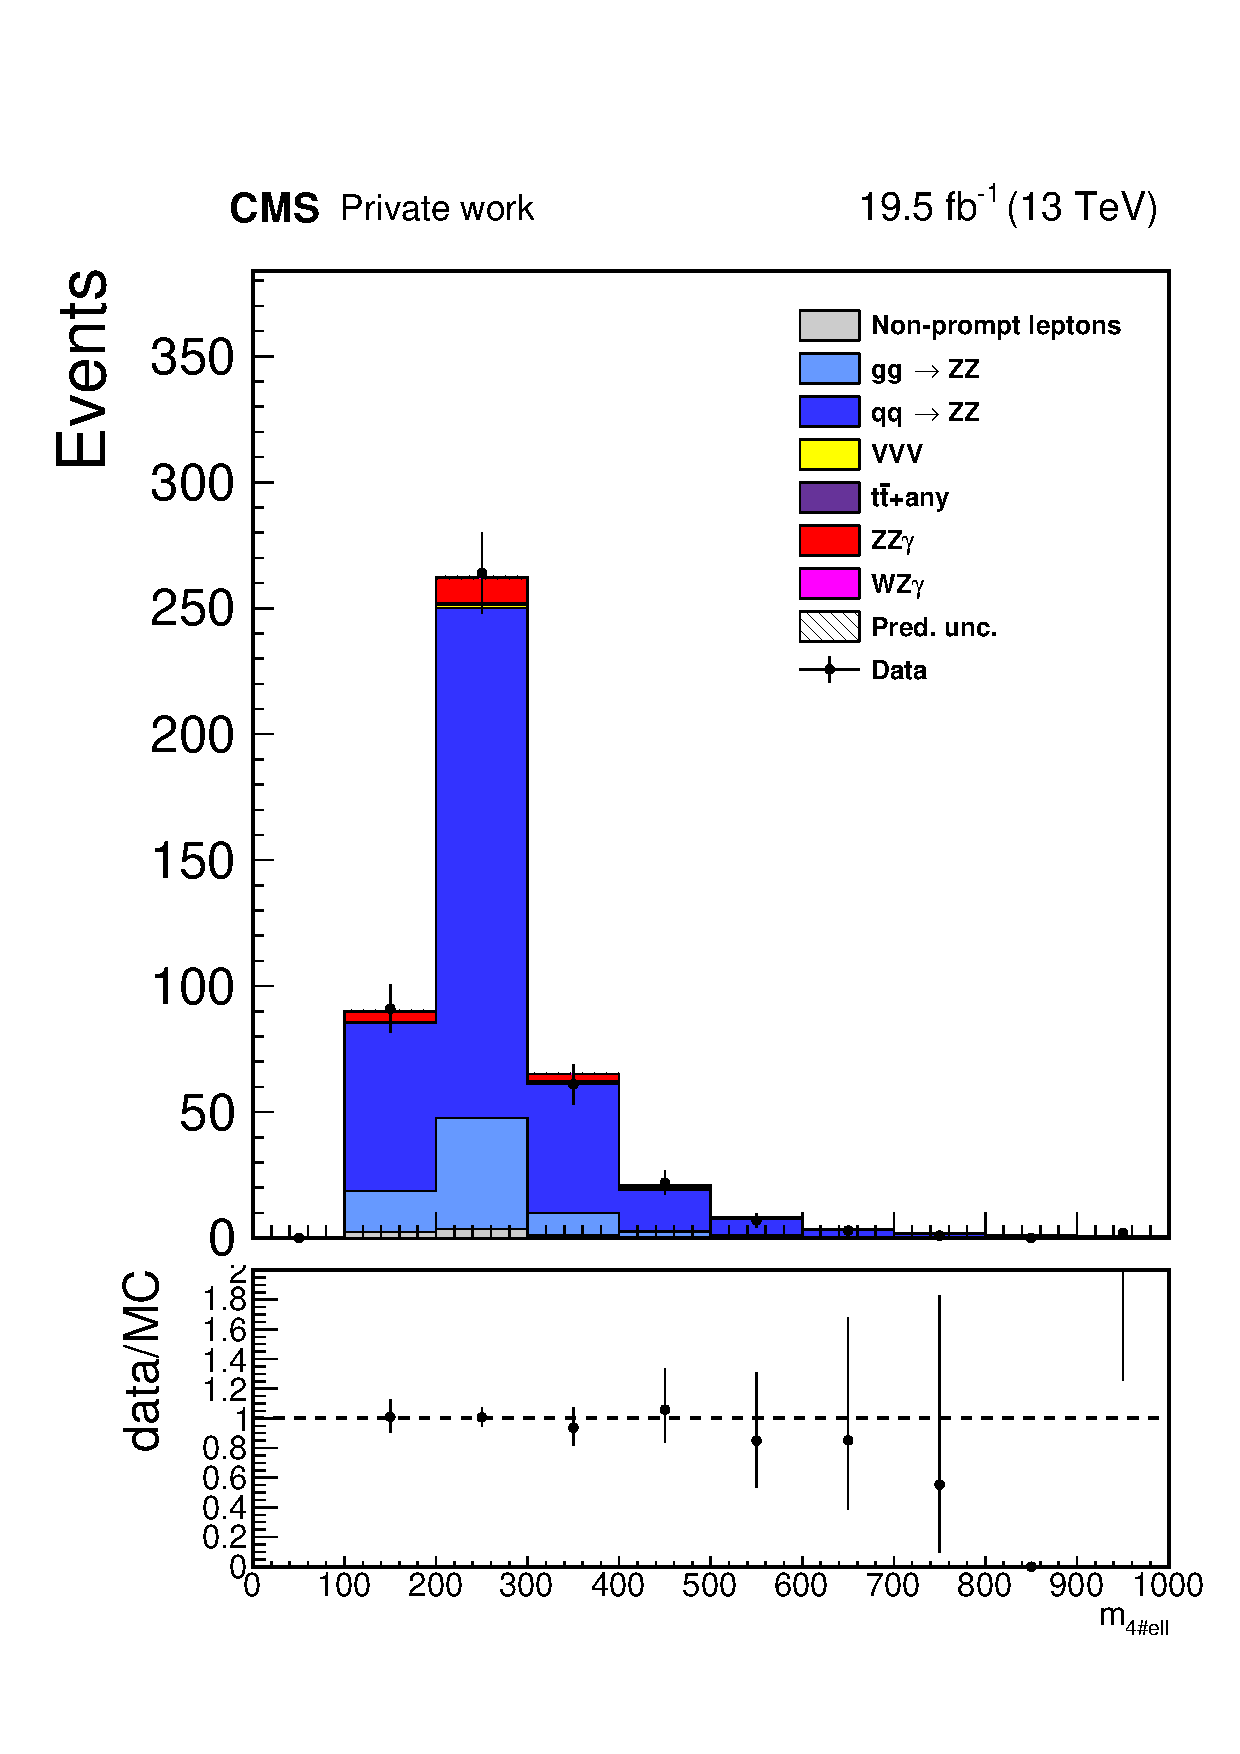
\includegraphics[width=.25\textwidth]{Figures/VVGammaAnalyzer/2016preVFP/lepCR/SR4P/ZZ_mass_pow.pdf}}%
\subfigure [2016postVFP] {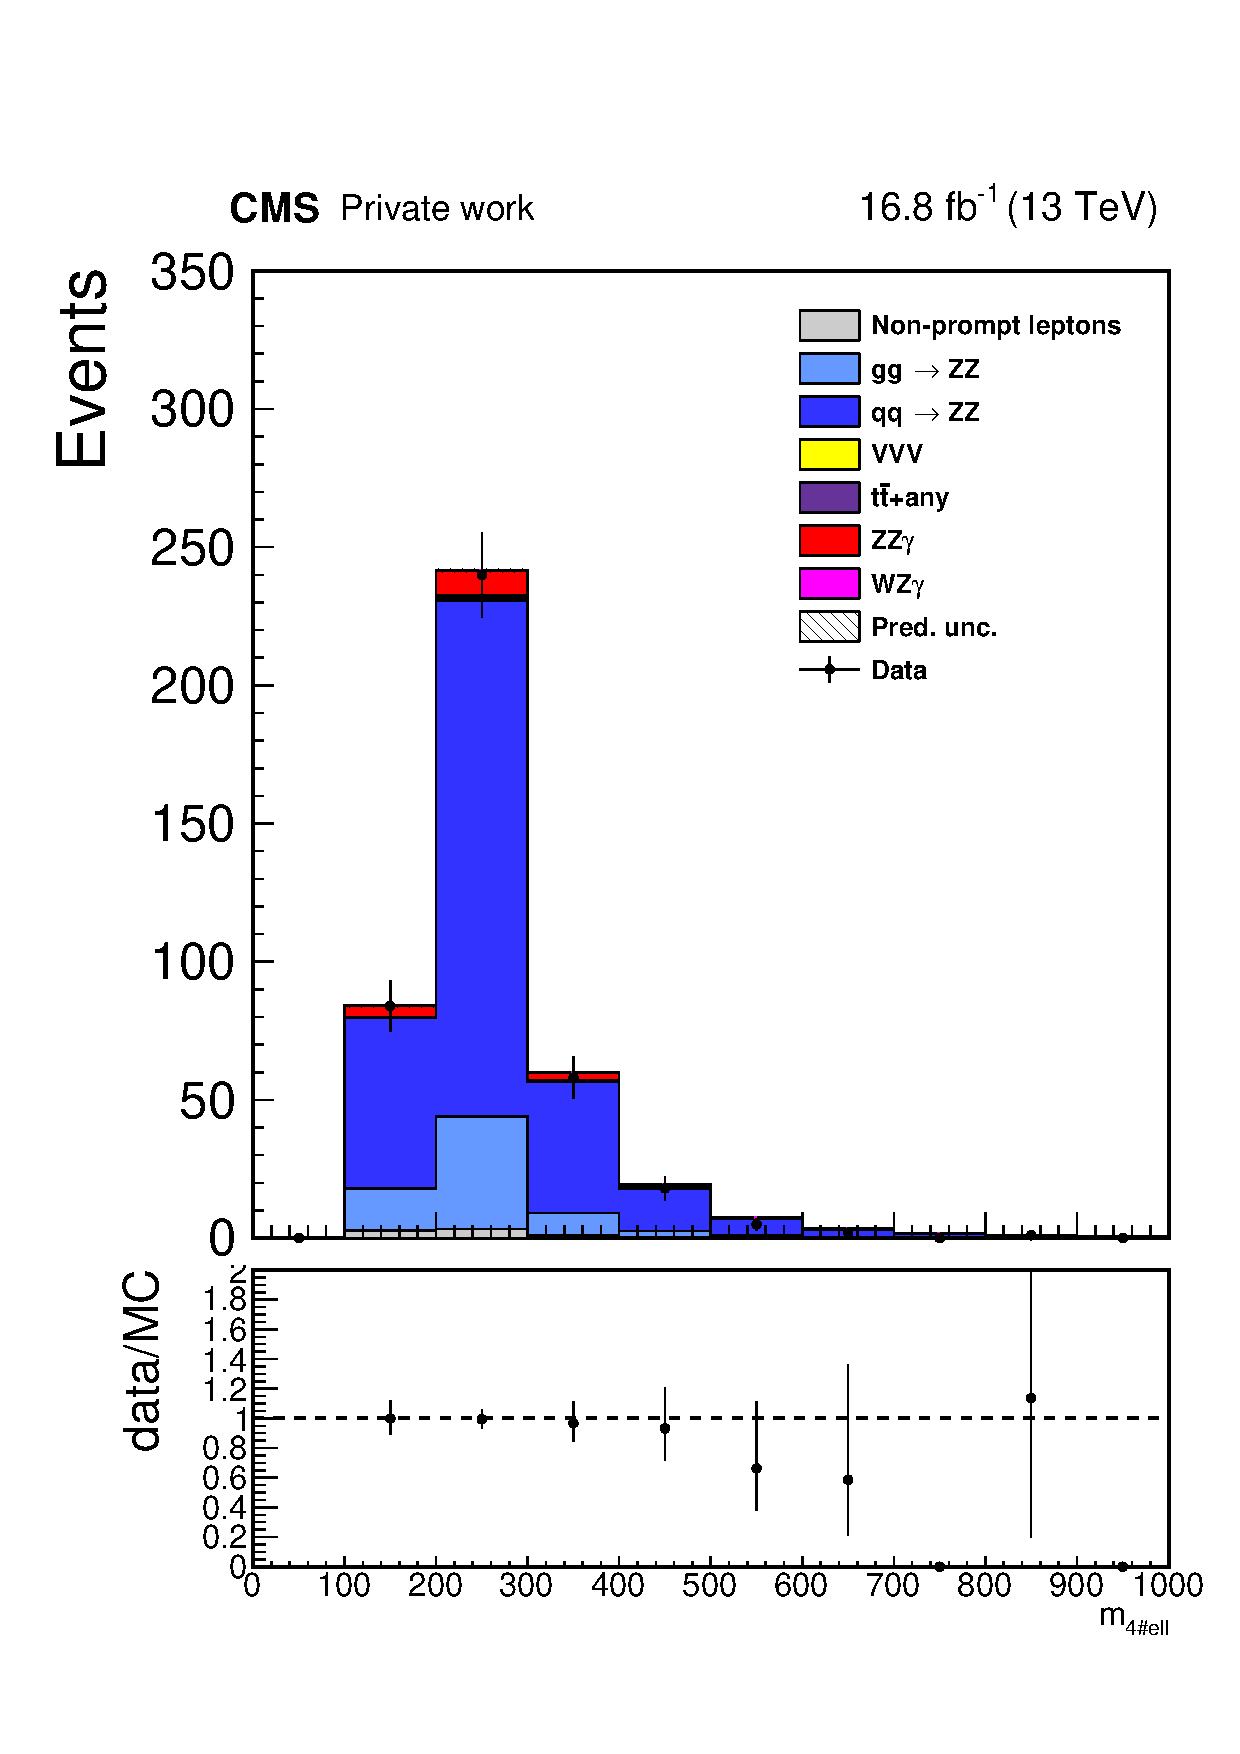
\includegraphics[width=.25\textwidth]{Figures/VVGammaAnalyzer/2016postVFP/lepCR/SR4P/ZZ_mass_pow.pdf}}%
\subfigure [2017       ] {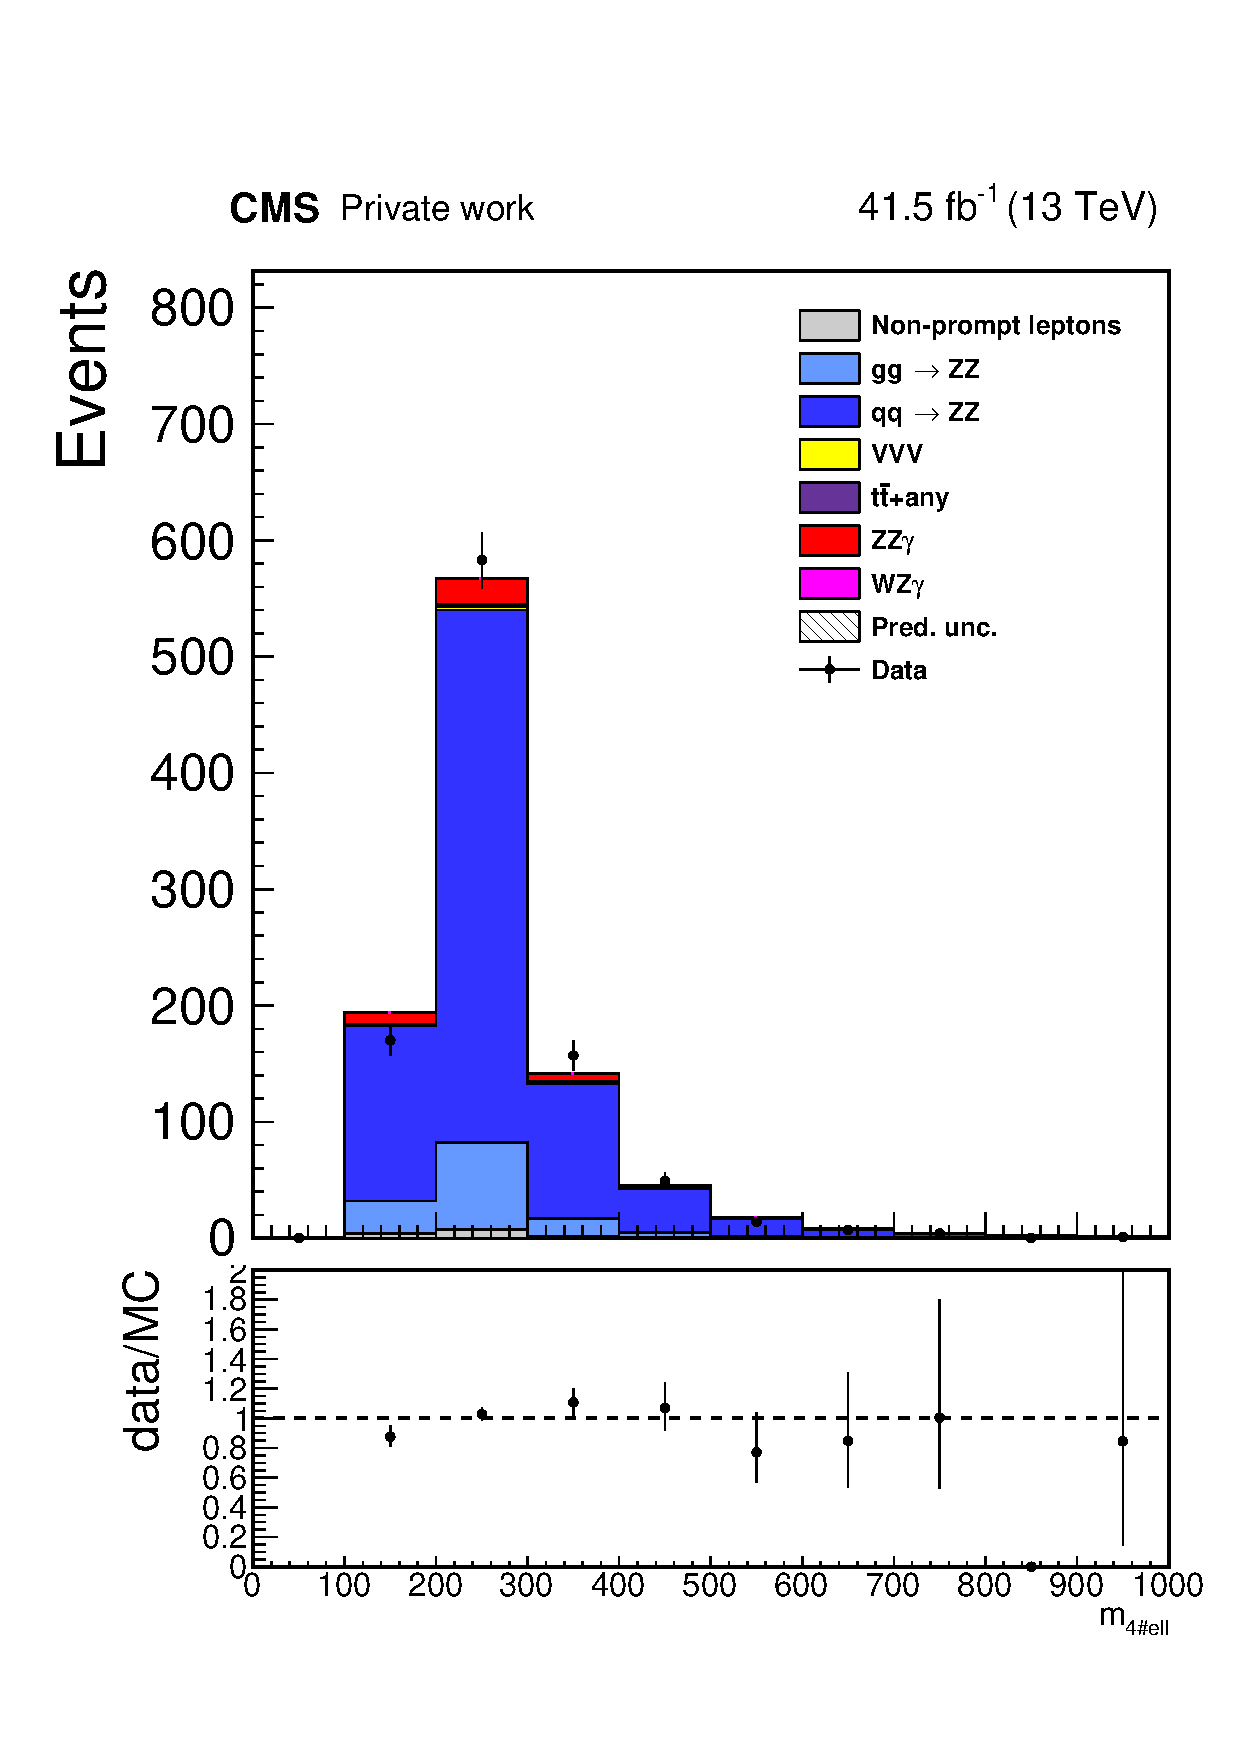
\includegraphics[width=.25\textwidth]{Figures/VVGammaAnalyzer/2017/lepCR/SR4P/ZZ_mass_pow.pdf}}%
\subfigure [2018       ] {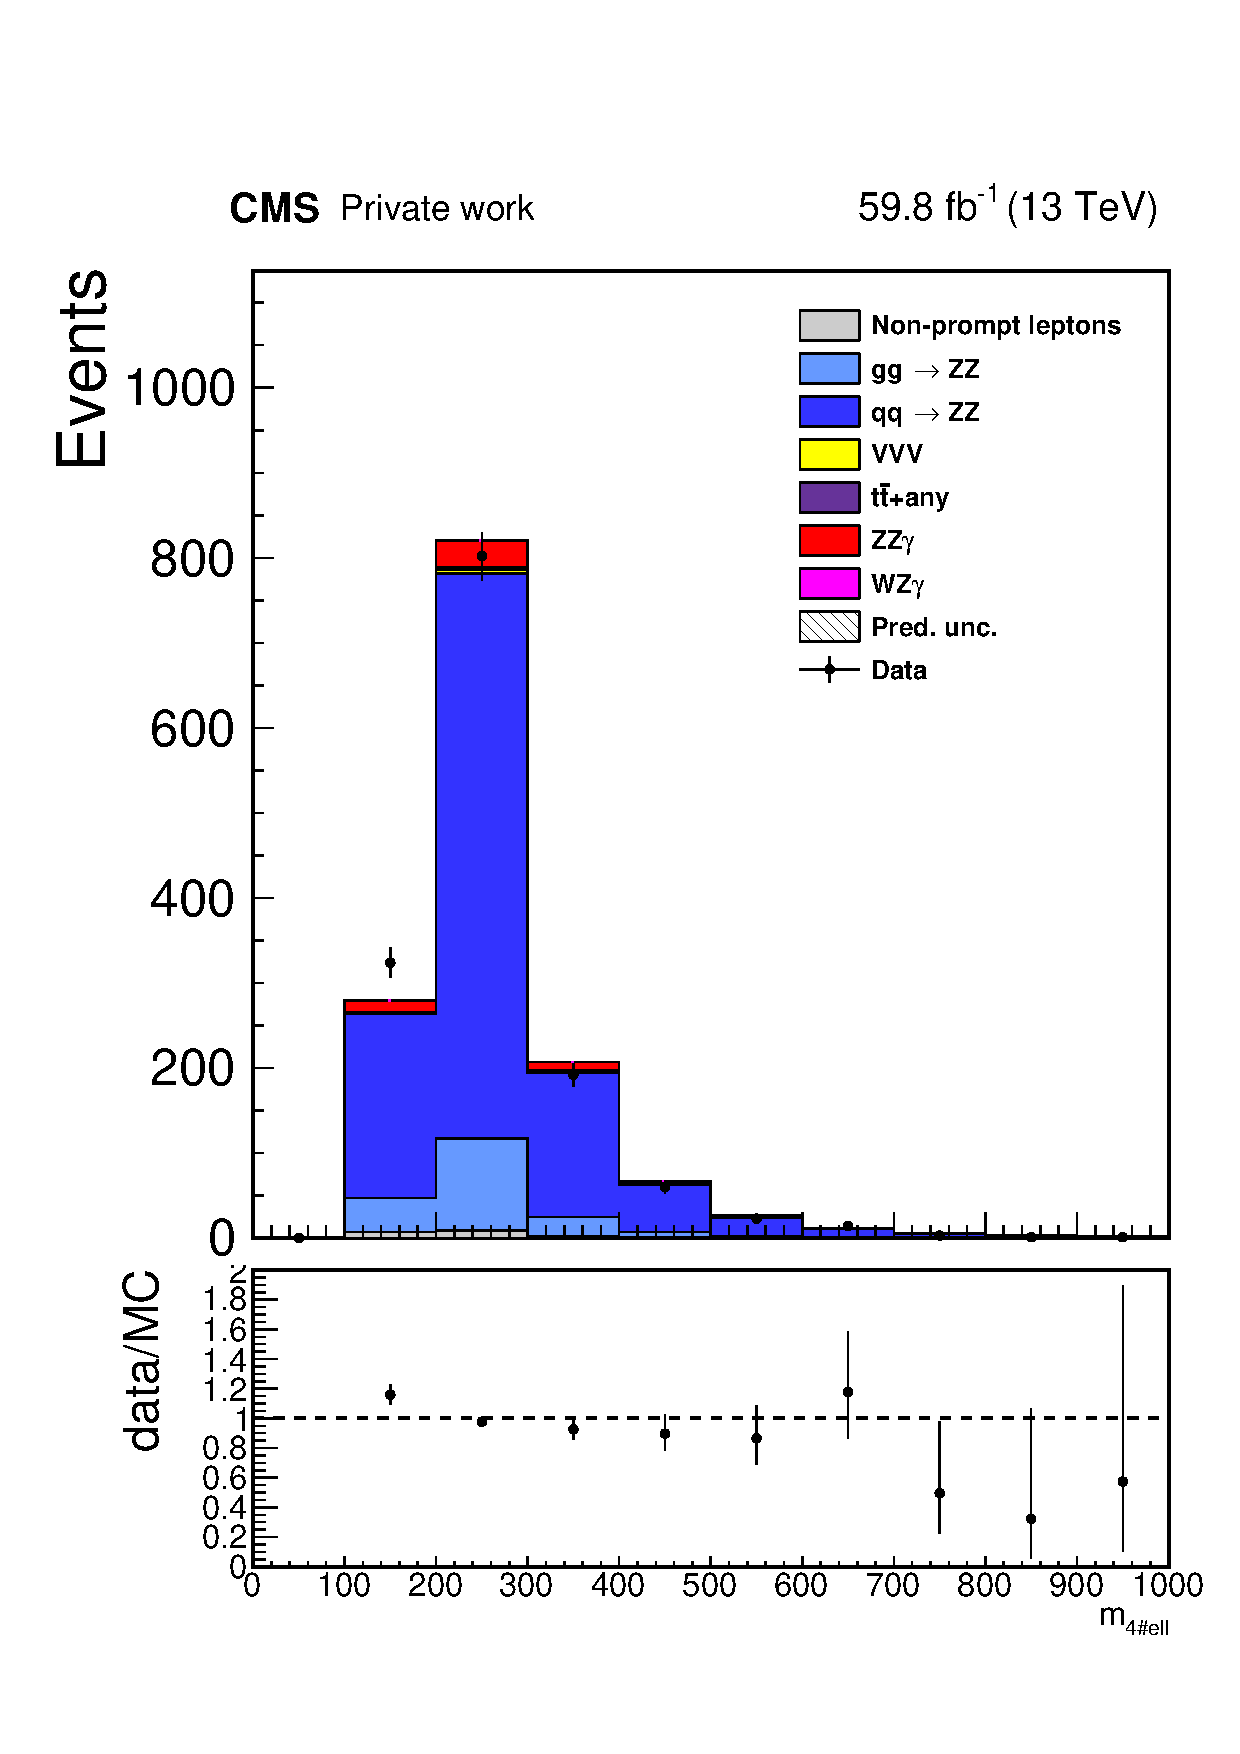
\includegraphics[width=.25\textwidth]{Figures/VVGammaAnalyzer/2018/lepCR/SR4P/ZZ_mass_pow.pdf}}
\caption{Invariant mass of the ZZ system, without any requirements on the presence of photons, for each of the data-taking periods of \Run2.}
\label{fig:ZZmass_byyear}
\end{figure}

